% ---------------------------------------------------------------------
% Illustrative examples -- experiment sections for the sample-path paper
%
% Contents:
%   1. "Sub-optimality bounds": restatement of the POMDP-level results
%      and their MDP specializations, with the document's own numbering:
%        Theorem 1  (abs, POMDP)   = Theorem 2  of the CDC paper
%                                    (docs/pdf/sample_path_cdc.pdf)
%        Theorem 2  (signed, POMDP)= Theorem 1  of the signed-bound note
%                                    (docs/pdf/signed_bound_last.pdf)
%        Remark 1   (lower collapse)= Remark 1  of the signed-bound note
%        Corollary 1 (abs, MDP)    = Corollary 4 of the CDC paper
%        Corollary 2 (signed, MDP) = new MDP specialization of the
%                                    signed theorem
%   2. Approximate Inventory Management (abs + signed computations)
%   3. Approximate Remote Transmission Scheduling (abs + signed)
%
% Figures are produced by notebooks/Finite_Horizon_Bounds.ipynb and
% notebooks/IoT_Bounds.ipynb and saved under figures/,
% figures/finite_horizon/, and figures/iot/.
% ---------------------------------------------------------------------
\documentclass[10pt]{article}
\usepackage[margin=1in]{geometry}
\usepackage{amsmath, amssymb, amsthm}
\usepackage{graphicx}
\usepackage{subcaption}
\graphicspath{{../../figures/}{../../figures/finite_horizon/}{../../figures/iot/}}

\newtheorem{theorem}{Theorem}
\newtheorem{corollary}{Corollary}
\newtheorem{remark}{Remark}
\theoremstyle{definition}
\newtheorem{assumption}{Assumption}

\newcommand{\clip}[1]{\left[#1\right]_{-B}^{B}}
\newcommand{\clipS}[1]{\left[#1\right]_{-S_{\max}}^{S_{\max}}}
\newcommand{\Dsgn}{\Delta^{\mathrm{sgn}}}

\begin{document}

\section*{Sub-optimality bounds}

For convenience, we first restate the sub-optimality bounds that the
experiments illustrate: the absolute-value bound and the signed bound,
both in their general (POMDP) form, followed by the MDP corollaries
that are used in the computations.

Consider a POMDP $\mathcal{P}$ over a finite horizon $T$. At each time
$t$ the controller has access to the history
$h_t = (y_{1:t}, a_{1:t-1}) \in \mathcal{H}_t$, selects an action
$a_t \in \mathcal{A}$, and incurs a per-step cost $c_t(h_t, a_t)$. Let
$(V^\star_t, \pi^\star_t)$ denote the optimal value function and an
optimal policy of $\mathcal{P}$. An AIS generator
$(\sigma_t, \hat c_t, \hat P_t)_{t=1}^{T}$ compresses the history into
$z_t = \sigma_t(h_t) \in \mathcal{Z}$ and defines an approximate MDP
with optimal value functions $(\hat V^\star_t, \hat Q^\star_t)$ and
optimal policy $\hat\pi^\star_t : \mathcal{Z} \to \mathcal{A}$,
computed by backward induction. The deployed policy is the AIS-optimal
policy lifted to $\mathcal{P}$,
$\pi_t(h_t) = \hat\pi^\star_t(\sigma_t(h_t))$, with value function
$V^{\hat\pi^\star}_t$. Finally, let
$\nu_t(\cdot\,|h_t, a) = \mathbb{P}(\sigma_{t+1}(H_{t+1}) \in \cdot\,|
h_t, a)$ denote the true conditional distribution of the next AIS.

\begin{assumption}[cost mismatch]\label{ass:eps}
For each $t \in \{1, \dots, T\}$, there exists a measurable function
$\varepsilon_t : \mathcal{H}_t \times \mathcal{A} \to \mathbb{R}_{\ge 0}$
such that for all $h_t \in \mathcal{H}_t$ and $a \in \mathcal{A}$,
\[
\bigl|c_t(h_t, a) - \hat c_t(\sigma_t(h_t), a)\bigr|
\le \varepsilon_t(h_t, a).
\]
\end{assumption}

\begin{assumption}[transition mismatch]\label{ass:delta}
For each $t \in \{1, \dots, T-1\}$, there exists a measurable function
$\Delta_t : \mathcal{H}_t \times \mathcal{A} \to \mathbb{R}_{\ge 0}$
such that for all $h_t \in \mathcal{H}_t$ and $a \in \mathcal{A}$,
\[
\Bigl|\int \hat V^\star_{t+1}(z_{t+1})\, \nu_t(dz_{t+1}|h_t, a)
- \int \hat V^\star_{t+1}(z_{t+1})\,
  \hat P_t(dz_{t+1}|\sigma_t(h_t), a)\Bigr|
\le \Delta_t(h_t, a).
\]
\end{assumption}

\begin{theorem}[absolute-value bound]\label{thm:abs-pomdp}
Suppose that for each $t \in \{1, \dots, T\}$, there exist measurable
functions $\alpha_t : \mathcal{H}_t \to \mathbb{R}$ and
$\beta_t : \mathcal{H}_t \times \mathcal{A} \to \mathbb{R}$ such that
$\beta_T(h_T, a_T) \ge \varepsilon_T(h_T, a_T)$ and for $t < T$:
\begin{equation}
\beta_t(h_t, a_t) \ge \varepsilon_t(h_t, a_t)
+ \int \alpha_{t+1}(h_t, a_t, y_{t+1})\, P(dy_{t+1}|h_t, a_t)
+ \Delta_t(h_t, a_t),
\label{eq:abs-rec}
\end{equation}
and for all $t \in \{1, \dots, T\}$:
\begin{equation}
\alpha_t(h_t) \ge \max\bigl\{\beta_t(h_t, \pi^\star_t(h_t)),\;
\beta_t(h_t, \hat\pi^\star_t(\sigma_t(h_t)))\bigr\}.
\label{eq:abs-anchor}
\end{equation}
Then, under Assumptions~\ref{ass:eps} and~\ref{ass:delta}, for all
$t \in \{1, \dots, T\}$ and all $h_t \in \mathcal{H}_t$, the AIS-based
policy $\pi_t(h_t) = \hat\pi^\star_t(\sigma_t(h_t))$ satisfies
\[
V^{\hat\pi^\star}_t(h_t) - V^\star_t(h_t) \le 2\alpha_t(h_t).
\]
\end{theorem}

The signed bound does not bound the magnitudes of the two mismatches
separately; instead it propagates the \emph{signed} one-step mismatch
\begin{equation}
\Dsgn_t(h_t, a_t)
= \Bigl[c_t(h_t, a_t)
  + \int \hat V^\star_{t+1}\, d\nu_t(\cdot\,|h_t, a_t)\Bigr]
- \Bigl[\hat c_t(\sigma_t(h_t), a_t)
  + \int \hat V^\star_{t+1}\, d\hat P_t(\cdot\,|\sigma_t(h_t), a_t)\Bigr],
\label{eq:sgn-mismatch-pomdp}
\end{equation}
with $\hat V^\star_{T+1} \equiv 0$ (so that
$\Dsgn_T = c_T - \hat c_T$). Under Assumptions~\ref{ass:eps}
and~\ref{ass:delta}, $|\Dsgn_t| \le \varepsilon_t + \Delta_t$, but
$\Dsgn_t$ retains cancellations between the cost and kernel mismatches.
It tracks \emph{two} signed error streams, both measured against the
shared baseline $\hat V^\star$: a policy-evaluation stream
$\alpha^{\hat\pi^\star}_t$ (over-estimating
$V^{\hat\pi^\star}_t - \hat V^\star_t \circ \sigma_t$) and an
optimality stream $\alpha^\star_t$ (under-estimating
$V^\star_t - \hat V^\star_t \circ \sigma_t$).

\begin{theorem}[signed bound]\label{thm:sgn-pomdp}
Suppose that for each $t \in \{1, \dots, T\}$, there exist measurable
functions $\alpha^{\hat\pi^\star}_t, \alpha^\star_t : \mathcal{H}_t \to
\mathbb{R}$ and $\beta^{\hat\pi^\star}_t, \beta^\star_t : \mathcal{H}_t
\times \mathcal{A} \to \mathbb{R}$ such that
\begin{equation}
\beta^{\hat\pi^\star}_T(h_T, a_T) \ge \Dsgn_T(h_T, a_T)
\ge \beta^\star_T(h_T, a_T),
\label{eq:sgn-terminal-pomdp}
\end{equation}
and for $t < T$:
\begin{equation}
\begin{aligned}
\beta^{\hat\pi^\star}_t(h_t, a_t) &\ge \Dsgn_t(h_t, a_t)
+ \int \alpha^{\hat\pi^\star}_{t+1}(h_t, a_t, y_{t+1})\,
  P(dy_{t+1}|h_t, a_t),\\
\beta^{\star}_t(h_t, a_t) &\le \Dsgn_t(h_t, a_t)
+ \int \alpha^{\star}_{t+1}(h_t, a_t, y_{t+1})\,
  P(dy_{t+1}|h_t, a_t),
\end{aligned}
\label{eq:sgn-rec-pomdp}
\end{equation}
and for all $t \in \{1, \dots, T\}$:
\begin{equation}
\alpha^{\hat\pi^\star}_t(h_t)
\ge \beta^{\hat\pi^\star}_t\bigl(h_t, \hat\pi^\star_t(\sigma_t(h_t))\bigr),
\qquad
\alpha^{\star}_t(h_t)
\le \beta^{\star}_t\bigl(h_t, \pi^\star_t(h_t)\bigr).
\label{eq:sgn-anchor-pomdp}
\end{equation}
Then, for all $t \in \{1, \dots, T\}$ and all $h_t \in \mathcal{H}_t$,
the AIS-based policy $\pi_t(h_t) = \hat\pi^\star_t(\sigma_t(h_t))$
satisfies
\[
V^{\hat\pi^\star}_t(h_t) - V^\star_t(h_t)
\le \alpha^{\hat\pi^\star}_t(h_t) - \alpha^{\star}_t(h_t).
\]
\end{theorem}

\begin{remark}\label{rem:collapse}
Two comments on Theorem~\ref{thm:sgn-pomdp}. (i)~Choosing
$\alpha^{\hat\pi^\star}_t = \alpha_t$, $\alpha^\star_t = -\alpha_t$,
$\beta^{\hat\pi^\star}_t = \beta_t$, $\beta^\star_t = -\beta_t$
recovers the absolute-value bound of Theorem~\ref{thm:abs-pomdp} with
certificate $2\alpha_t$; the signed bound is therefore always at least
as tight. (ii)~Reversing every inequality
in~\eqref{eq:sgn-terminal-pomdp}--\eqref{eq:sgn-anchor-pomdp} --- which
also moves the $\star$-anchor in~\eqref{eq:sgn-anchor-pomdp} from
$\pi^\star_t(h_t)$ to $\hat\pi^\star_t(\sigma_t(h_t))$ --- yields a
symmetric \emph{lower} bound $V^{\hat\pi^\star}_t - V^\star_t \ge
\alpha^{\hat\pi^\star}_t - \alpha^\star_t$. This lower bound is not
informative: with the $\star$-anchor forced to $\hat\pi^\star$, both
streams satisfy the identical recursion with the same mismatch, kernel,
and terminal value, so their tightest admissible choices coincide and
the certified lower bound collapses to the trivial
$V^{\hat\pi^\star}_t - V^\star_t \ge 0$.
\end{remark}

\subsection*{MDP specialization}

In the fully observed setting, the POMDP reduces to an MDP: the
observation equals the state ($Y_t = S_t$), the history compression is
the identity on the current state ($\sigma_t(h_t) = s_t$,
$\mathcal{Z} = \mathcal{S}$), and
$\nu_t(\cdot\,|h_t, a) = P_t(\cdot\,|s_t, a)$. We compare two
finite-horizon MDPs $\mathcal{M} = \langle \mathcal{S}, \mathcal{A},
\{P_t\}, \{c_t\}, T\rangle$ and $\hat{\mathcal{M}} = \langle
\mathcal{S}, \mathcal{A}, \{\hat P_t\}, \{\hat c_t\}, T\rangle$ on the
same state and action spaces. Assumptions~\ref{ass:eps}
and~\ref{ass:delta} then read: there exist
$\varepsilon_t, \Delta_t : \mathcal{S} \times \mathcal{A} \to
\mathbb{R}_{\ge 0}$ such that
\[
|c_t(s,a) - \hat c_t(s,a)| \le \varepsilon_t(s,a),
\qquad
\Bigl|\sum_{s'} \hat V^\star_{t+1}(s')
\bigl[P_t(s'|s,a) - \hat P_t(s'|s,a)\bigr]\Bigr| \le \Delta_t(s,a).
\]

\begin{corollary}[MDP, absolute-value bound]\label{cor:abs-mdp}
Under Assumptions~\ref{ass:eps} and~\ref{ass:delta} (in their MDP form
above), suppose that for each $t \in \{1, \dots, T\}$, there exist
measurable functions $\alpha_t : \mathcal{S} \to \mathbb{R}$ and
$\beta_t : \mathcal{S} \times \mathcal{A} \to \mathbb{R}$ such that
$\beta_T(s,a) \ge \varepsilon_T(s,a)$ and for $t < T$:
\begin{equation}
\beta_t(s,a) \ge \varepsilon_t(s,a)
+ \sum_{s'} \alpha_{t+1}(s')\, P_t(s'|s,a) + \Delta_t(s,a),
\label{eq:cor-abs-rec}
\end{equation}
and for all $t \in \{1, \dots, T\}$:
\begin{equation}
\alpha_t(s) \ge \max\bigl\{\beta_t(s, \pi^\star_t(s)),\;
\beta_t(s, \hat\pi^\star_t(s))\bigr\}.
\label{eq:cor-abs-anchor}
\end{equation}
Then, the policy $\pi_t(s) = \hat\pi^\star_t(s)$ satisfies for all $t$
and $s$:
\[
|V^{\hat\pi^\star}_t(s) - V^\star_t(s)| \le 2\alpha_t(s).
\]
\end{corollary}

\begin{corollary}[MDP, signed bound]\label{cor:sgn-mdp}
Define the signed one-step mismatch
\begin{equation}
\Dsgn_t(s,a) = \bigl[c_t(s,a) - \hat c_t(s,a)\bigr]
+ \sum_{s'} \hat V^\star_{t+1}(s')
  \bigl[P_t(s'|s,a) - \hat P_t(s'|s,a)\bigr],
\label{eq:cor-sgn-mismatch}
\end{equation}
with $\hat V^\star_{T+1} \equiv 0$. Suppose that for each
$t \in \{1, \dots, T\}$, there exist measurable functions
$\alpha^{\hat\pi^\star}_t, \alpha^\star_t : \mathcal{S} \to \mathbb{R}$
and $\beta^{\hat\pi^\star}_t, \beta^\star_t : \mathcal{S} \times
\mathcal{A} \to \mathbb{R}$ such that
\begin{equation}
\beta^{\hat\pi^\star}_T(s,a) \ge \Dsgn_T(s,a) \ge \beta^\star_T(s,a),
\label{eq:cor-sgn-terminal}
\end{equation}
and for $t < T$:
\begin{align}
\beta^{\hat\pi^\star}_t(s,a) &\ge \Dsgn_t(s,a)
+ \sum_{s'} \alpha^{\hat\pi^\star}_{t+1}(s')\, P_t(s'|s,a),
\label{eq:cor-sgn-rec-ph}\\
\beta^{\star}_t(s,a) &\le \Dsgn_t(s,a)
+ \sum_{s'} \alpha^{\star}_{t+1}(s')\, P_t(s'|s,a),
\label{eq:cor-sgn-rec-star}
\end{align}
and for all $t \in \{1, \dots, T\}$:
\begin{align}
\alpha^{\hat\pi^\star}_t(s)
&\ge \beta^{\hat\pi^\star}_t\bigl(s, \hat\pi^\star_t(s)\bigr),
\label{eq:cor-sgn-anchor-ph}\\
\alpha^{\star}_t(s)
&\le \beta^{\star}_t\bigl(s, \pi^\star_t(s)\bigr).
\label{eq:cor-sgn-anchor-star}
\end{align}
Then, the policy $\pi_t(s) = \hat\pi^\star_t(s)$ satisfies for all $t$
and $s$:
\[
V^{\hat\pi^\star}_t(s) - V^\star_t(s)
\le \alpha^{\hat\pi^\star}_t(s) - \alpha^{\star}_t(s).
\]
\end{corollary}

Corollary~\ref{cor:abs-mdp} follows from Theorem~\ref{thm:abs-pomdp}
and Corollary~\ref{cor:sgn-mdp} from Theorem~\ref{thm:sgn-pomdp} by
taking $Y_t = S_t$, $\sigma_t(h_t) = s_t$, and $\mathcal{Z} =
\mathcal{S}$; the integrals over the next observation become sums over
the next state, so
\eqref{eq:cor-abs-rec}--\eqref{eq:cor-abs-anchor} are the state-space
forms of \eqref{eq:abs-rec}--\eqref{eq:abs-anchor},
\eqref{eq:cor-sgn-mismatch} specializes
\eqref{eq:sgn-mismatch-pomdp}, and
\eqref{eq:cor-sgn-rec-ph}--\eqref{eq:cor-sgn-rec-star} specialize
\eqref{eq:sgn-rec-pomdp}.

\section*{Approximate Inventory Management}

We illustrate the results of Corollaries~\ref{cor:abs-mdp}
and~\ref{cor:sgn-mdp} on an inventory management problem. Consider an
inventory control MDP with state space
$\mathcal{S} = \{-S_{\max}, \dots, S_{\max}\}$, action space
$\mathcal{A} = \{0, 1, \dots, S_{\max}\}$, and dynamics
\[
S_{t+1} = \clipS{S_t + A_t - N_t},
\]
where $[\cdot]_{-S_{\max}}^{S_{\max}}$ clips its argument to
$[-S_{\max}, S_{\max}]$ and the demand $N_t$ is an i.i.d.\
$\text{Binomial}(n, q)$ process. Let the per-step cost be
$c(s,a) = p\,a + h(s)$, where
\[
h(s) =
\begin{cases}
  c_h\, s & s \ge 0,\\
  -c_s\, s & s < 0,
\end{cases}
\]
$p$ is the per-unit ordering cost, $c_h$ is the holding cost, and $c_s$
is the shortage cost. The system runs for an infinite horizon and future
is discounted by a factor $\gamma \in (0,1)$. We parameterize such a
model as $\mathcal{M} = (S_{\max}, \gamma, n, q, c_h, c_s, p)$.

To apply Corollaries~\ref{cor:abs-mdp} and~\ref{cor:sgn-mdp} directly,
we reformulate the problem as a finite-horizon MDP with horizon $T$
(for some large $T$) by absorbing the discount factor into a
time-varying cost $c_t(s,a) = \gamma^{t-1}\bigl[p\,a + h(s)\bigr]$ for
$t = 1, \dots, T$, and similarly for the approximate model. The
transitions remain stationary: $P_t = P$ and $\hat P_t = \hat P$ for
all~$t$.

We consider the following two models:
\begin{itemize}
  \item True model \phantom{Approx.\ }$\mathcal{M} = (500, 0.75, 10, 0.4, 4.0, 2, 5)$.
  \item Approx.\ model $\hat{\mathcal{M}} = (500, 0.75, 10, 0.5, 3.8, 2, 5)$.
\end{itemize}
Furthermore, Assumption~\ref{ass:eps} is satisfied with
$\varepsilon_t(s,a) = \gamma^{t-1}\varepsilon(s)$, where
$\varepsilon(s) = |h_{\mathcal{M}}(s) - h_{\hat{\mathcal{M}}}(s)|$
depends only on the state since the ordering cost $p$ is identical in
both models. Explicitly,
\[
\varepsilon(s) =
\begin{cases}
  |c_h - \hat c_h| \cdot s = 0.2\,s & s \ge 0,\\
  |c_s - \hat c_s| \cdot |s| = 0 & s < 0.
\end{cases}
\]
Also, Assumption~\ref{ass:delta} is satisfied with
\[
\Delta_t(s,a) = \Bigl|\sum_{s'} \hat V^\star_{t+1}(s')
  \bigl[P(s'|s,a) - \hat P(s'|s,a)\bigr]\Bigr|,
\]
where $\hat V^\star_{t+1}$ is the time-$(t{+}1)$ optimal value function
of $\hat{\mathcal{M}}$, computed by backward induction. Both
$\varepsilon_t$ and $\Delta_t$ can be computed exactly since the state
and action spaces are finite.

\subsection*{Absolute-value bound (Corollary~\ref{cor:abs-mdp})}

We define $\alpha, \beta$ functions satisfying the conditions of
Corollary~\ref{cor:abs-mdp} as follows. At the terminal time,
$\beta_T(s,a) = \gamma^{T-1}\varepsilon(s)$ and
$\alpha_T(s) = \gamma^{T-1}\varepsilon(s)$. For $t < T$:
\begin{equation}
\begin{aligned}
\beta_t(s,a) &= \gamma^{t-1}\varepsilon(s)
  + \sum_{s'} \alpha_{t+1}(s') P(s'|s,a) + \Delta_t(s,a),\\
\alpha_t(s) &= \max_{a \in A(s)} \beta_t(s,a),
\end{aligned}
\label{eq:inv-alpha-beta}
\end{equation}
where $A(s)$ is the action set we will determine below; these choices
satisfy~\eqref{eq:cor-abs-rec} with equality
and~\eqref{eq:cor-abs-anchor} whenever $A(s)$ contains both
$\pi^\star_t(s)$ and $\hat\pi^\star_t(s)$. Corollary~\ref{cor:abs-mdp}
then implies
\begin{equation}
V^{\hat\pi^\star}_1(s) - 2\alpha_1(s)
\;\le\; V^\star_1(s) \;\le\; V^{\hat\pi^\star}_1(s).
\label{eq:inv-sandwich}
\end{equation}

As given in~\eqref{eq:cor-abs-anchor}, the tightest bound uses
\begin{equation}
A(s) = \{\pi^\star_t(s), \hat\pi^\star_t(s)\},
\label{eq:inv-Amax}
\end{equation}
which requires the true model's optimal policy. Since the optimal
policy is base-stock with level\footnote{Ordering above the maximum
demand is never optimal, as it guarantees positive inventory without
reducing shortage risk.} $s^\star_t \le n = 10$, the restricted action
set
\begin{equation}
A_{\mathrm{res}}(s)
= \bigl\{\max(0,\, s^\star - s) : s^\star \in \{0, \dots, n\}\bigr\}
  \;\cup\; \{\hat\pi^\star_t(s)\}
\label{eq:inv-Ares}
\end{equation}
contains at most $n + 2 = 12$ actions and includes $\pi^\star_t(s)$
without requiring its explicit computation. This yields a bound nearly
as tight as the two-action variant while requiring only structural
knowledge of the policy class. We use $2\alpha^{\max}_1(s)$ and
$2\alpha^{\mathrm{res}}_1(s)$ to denote the sub-optimality bounds
in~\eqref{eq:inv-alpha-beta} when using the action set $A(s)$
from~\eqref{eq:inv-Amax} and~\eqref{eq:inv-Ares}, respectively.

We compare the sample-path bound in~\eqref{eq:inv-sandwich} with the
infinite-horizon sup-norm and weighted-norm bounds of [14]. Because the
distance between the finite- and discounted infinite-horizon objectives
is bounded by $\gamma^T \|c\|_\infty/(1-\gamma)$, the value functions at
$t = 1$ agree to numerical precision (at $T = 100$ and $\gamma = 0.75$,
$\gamma^T < 10^{-12}$). For both models, we compute $V^\star_t$,
$\hat V^\star_t$, $\pi^\star_t$, $\hat\pi^\star_t$ via backward
induction, and $V^{\hat\pi^\star}_1$ via policy evaluation. All three
bounds are plotted in Fig.~\ref{fig:inv-bounds}\subref{fig:inv-out}
(full state space) and Fig.~\ref{fig:inv-bounds}\subref{fig:inv-in}
(zoomed into the region $\{-10, \dots, 10\}$). The shaded region
between $V^{\hat\pi^\star}_1(s)$ and the tightest lower bound indicates
where $V^\star_1(s)$ must lie.

The sample-path bound using $2\alpha^{\mathrm{res}}_1(s)$ is
substantially tighter than both existing bounds in the operating
region. At $s = 3$, the sample-path bound gives
$2\alpha^{\mathrm{res}}_1(3) = 42.31$ while the weighted-norm bound
gives $62.25$; at $s = 10$, the values are $33.78$ versus $83.46$.
Both are well below the sup-norm bound of $891.20$.

Fig.~\ref{fig:inv-max-vs-res} compares $2\alpha^{\max}_1(s)$ with
$2\alpha^{\mathrm{res}}_1(s)$. As can be seen from the figure, the
bounds are very close, confirming that the restricted action set
captures most of the tightening without requiring computation of the
true optimal policy.

\subsection*{Signed bound (Corollary~\ref{cor:sgn-mdp})}

The functions in~\eqref{eq:inv-alpha-beta} are chosen so that the
hypotheses of Corollary~\ref{cor:abs-mdp} hold; the resulting
certificate is an \emph{absolute-value} bound, and the outer
maximization in~\eqref{eq:inv-alpha-beta} accumulates the magnitudes
$\varepsilon_t + \Delta_t$ regardless of their signs. The signed bound
of Corollary~\ref{cor:sgn-mdp} is obtained from \emph{different
recursions}: it propagates the two signed streams through the signed
mismatch~\eqref{eq:cor-sgn-mismatch}, which here reads
$\Dsgn_t(s,a) = \gamma^{t-1}\bigl(h_{\mathcal{M}}(s) -
h_{\hat{\mathcal{M}}}(s)\bigr) + \sum_{s'}\hat V^\star_{t+1}(s')
\bigl[P(s'|s,a) - \hat P(s'|s,a)\bigr]$, i.e.\ the quantities of
Assumptions~\ref{ass:eps} and~\ref{ass:delta} \emph{without} the
absolute values. With $\alpha^{\hat\pi^\star}_{T+1} \equiv
\alpha^\star_{T+1} \equiv 0$, we choose the two streams backward for
$t = T, \dots, 1$ as
\begin{equation}
\begin{aligned}
\alpha^{\hat\pi^\star}_t(s)
&= \Dsgn_t\bigl(s, \hat\pi^\star_t(s)\bigr)
  + \sum_{s'} \alpha^{\hat\pi^\star}_{t+1}(s')\,
    P\bigl(s'\mid s, \hat\pi^\star_t(s)\bigr),\\
\alpha^{\star}_t(s)
&= \min_{a \in \mathcal{C}(s)}\Bigl[\Dsgn_t(s,a)
  + \sum_{s'} \alpha^{\star}_{t+1}(s')\, P(s'\mid s, a)\Bigr].
\end{aligned}
\label{eq:inv-signed-streams}
\end{equation}
The policy-evaluation stream $\alpha^{\hat\pi^\star}$ is an exact
recursion anchored at the single known action $\hat\pi^\star_t(s)$ ---
no action search --- and satisfies~\eqref{eq:cor-sgn-terminal},
\eqref{eq:cor-sgn-rec-ph}, and~\eqref{eq:cor-sgn-anchor-ph} with
equality. The optimality stream $\alpha^\star$ must satisfy the
sub-solution anchor~\eqref{eq:cor-sgn-anchor-star} at the unknown true
optimal action; taking a \texttt{min} over a candidate set
$\mathcal{C}(s)$ \emph{guaranteed to contain} $\pi^\star_t(s)$
realizes~\eqref{eq:cor-sgn-rec-star} and~\eqref{eq:cor-sgn-anchor-star}
without ever identifying $\pi^\star$ exactly. The \texttt{min} (vs.\
the \texttt{max} of~\eqref{eq:inv-alpha-beta}) and the signed
mismatch~\eqref{eq:cor-sgn-mismatch} are the only structural
differences from the absolute-value computation.
Corollary~\ref{cor:sgn-mdp} then certifies the one-sided bound
\begin{equation}
V^{\hat\pi^\star}_1(s) - V^\star_1(s)
\;\le\; U(s) := \alpha^{\hat\pi^\star}_1(s) - \alpha^{\star}_1(s),
\qquad\text{hence}\qquad
V^{\hat\pi^\star}_1(s) - U(s) \;\le\; V^\star_1(s)
\;\le\; V^{\hat\pi^\star}_1(s),
\label{eq:inv-U}
\end{equation}
where the upper half of the sandwich is the trivial optimality of
$V^\star$. As in the absolute-value case we consider three candidate
sets: $\mathcal{C}(s) = \{\pi^\star_t(s)\}$ (denoted $U^{\max}$), the
feasible base-stock candidates of~\eqref{eq:inv-Ares} (denoted
$U^{\mathrm{res}}$),\footnote{Because the optimality stream takes a
\texttt{min}, the restricted candidate set must be capped to feasible
actions $a \le S_{\max}$; at extreme-negative states a base-stock level
may be unreachable in one step, and without the cap the \texttt{min}
could select an infeasible action.} and all feasible actions (denoted
$U^{\sup}$). Since a \texttt{min} over a smaller set is larger, the
same ordering $U^{\max} \le U^{\mathrm{res}} \le U^{\sup}$ holds.

As discussed in Remark~\ref{rem:collapse}, the symmetric lower-bound
counterpart of Corollary~\ref{cor:sgn-mdp} is not informative: its
hypotheses force the optimality stream to be a super-solution anchored
at $\hat\pi^\star$ --- the same action, mismatch, kernel, and terminal
value as the policy-evaluation stream --- so the two streams coincide
and the in-framework lower bound collapses to the trivial
$V^{\hat\pi^\star}_1 - V^\star_1 \ge 0$. We verify this numerically:
computing the $\hat\pi^\star$-anchored super-solution as an independent
backward recursion reproduces $\alpha^{\hat\pi^\star}$ bit-exactly at
every $(t,s)$. The informative certificate is therefore the upper bound
$U$ in~\eqref{eq:inv-U}.

At $T = 100$, all signed bounds are valid
($\min_s [U(s) - \mathrm{gap}(s)] \ge 0$ up to numerical tolerance
$\sim 10^{-13}$). Over the operating region $\{-7, \dots, 3\}$ the true
gap peaks at $2.01$, and the signed certificates give
$U^{\max}_1 = 2.06$, $U^{\mathrm{res}}_1 = 2.80$, and
$U^{\sup}_1 = 2.80$, versus $2\alpha^{\max}_1 = 41.45$,
$2\alpha^{\mathrm{res}}_1 = 42.46$, and $2\alpha^{\sup}_1 = 688.33$ for
the absolute-value bound --- a $15$--$20\times$ tightening without any
additional model knowledge. At the reference states of
Fig.~\ref{fig:inv-bounds}, $U^{\mathrm{res}}_1(3) = 2.09$ and
$U^{\mathrm{res}}_1(10) = 1.38$, compared with the absolute-value
values $42.31$ and $33.78$ quoted above. $U^{\max}$ essentially
recovers the true gap ($2.06$ vs.\ $2.01$), and the
no-true-$\pi^\star$ variant $U^{\mathrm{res}}$ stays within $40\%$ of
it. Fig.~\ref{fig:inv-signed} plots the signed certificate band
$[V^{\hat\pi^\star}_1 - U^{\mathrm{res}}_1,\, V^{\hat\pi^\star}_1]$
against the absolute-value and weighted-norm lower bounds in the
operating region.

\begin{figure}[t]
  \centering
  \begin{subfigure}[b]{0.48\linewidth}
    \centering
    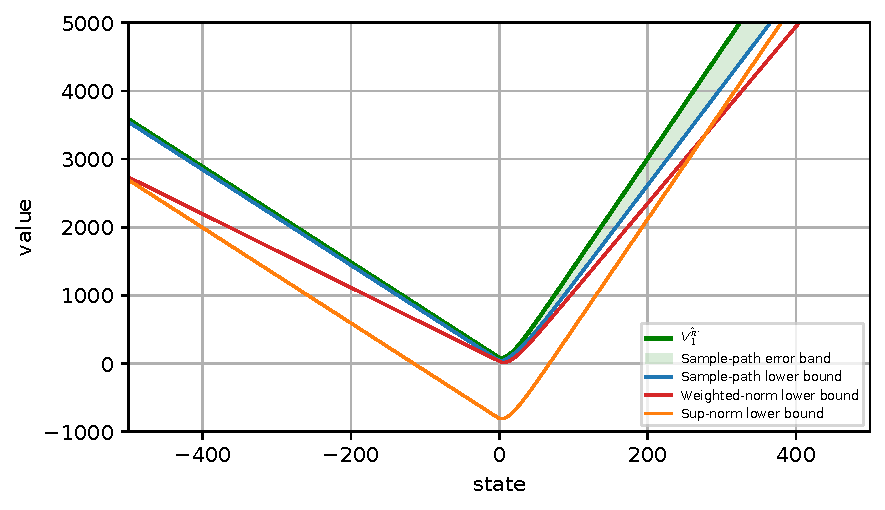
\includegraphics[width=\linewidth]{fh_bounds_comparison_out.pdf}
    \caption{entire state space}
    \label{fig:inv-out}
  \end{subfigure}
  \hfill
  \begin{subfigure}[b]{0.48\linewidth}
    \centering
    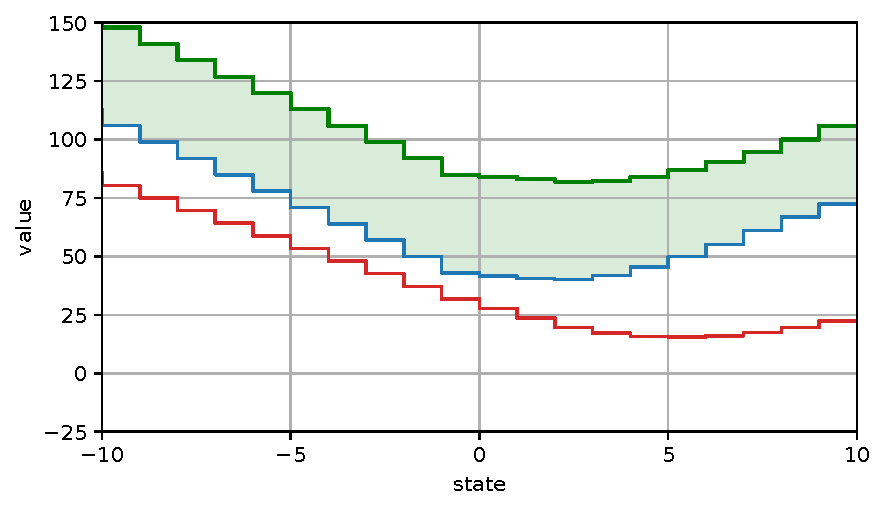
\includegraphics[width=\linewidth]{fh_bounds_comparison_in.pdf}
    \caption{zoomed in}
    \label{fig:inv-in}
  \end{subfigure}
  \caption{Comparison of lower bounds on $V^\star_1(s)$ for the
    finite-horizon inventory management model.}
  \label{fig:inv-bounds}
\end{figure}

\begin{figure}[t]
  \centering
  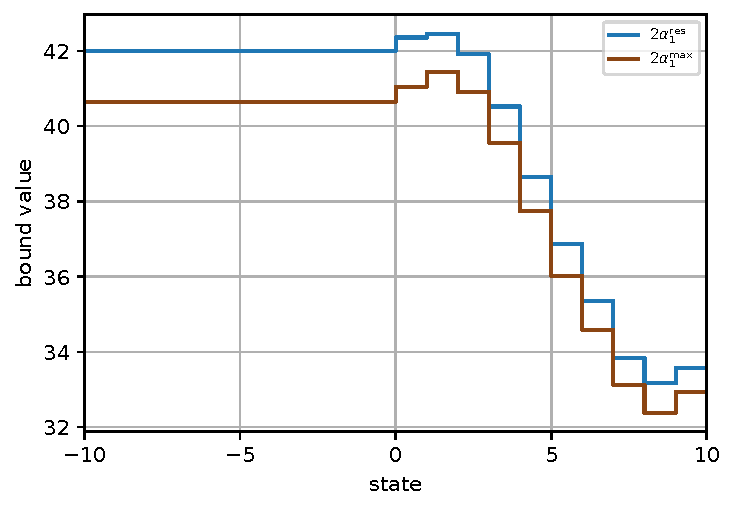
\includegraphics[width=0.6\linewidth]{fh_max_vs_res.pdf}
  \caption{Comparison of $2\alpha^{\max}_1(s)$ and
    $2\alpha^{\mathrm{res}}_1(s)$ in the region
    $s \in \{-10, \dots, 10\}$.}
  \label{fig:inv-max-vs-res}
\end{figure}

\begin{figure}[t]
  \centering
  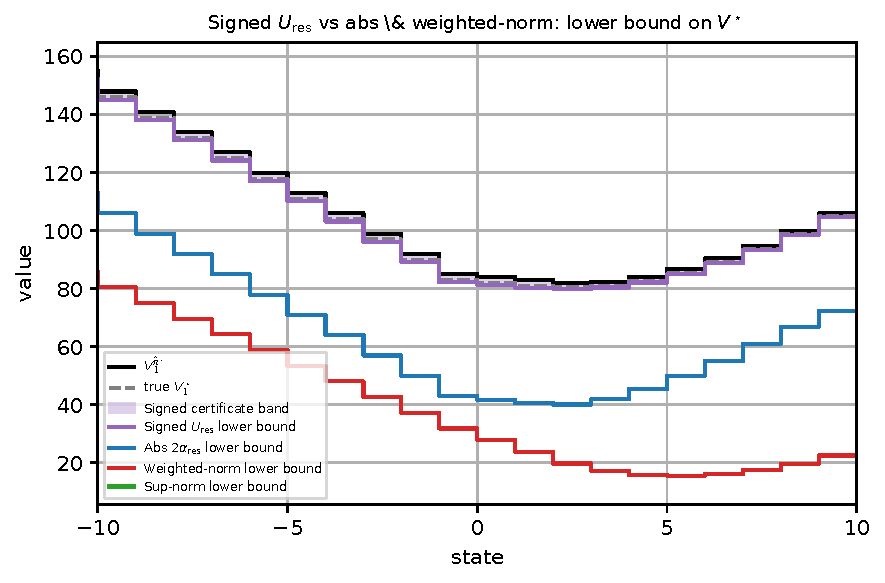
\includegraphics[width=0.6\linewidth]{signed_vs_abs_weighted_zoomed_in.pdf}
  \caption{Signed certificate band
    $[V^{\hat\pi^\star}_1 - U^{\mathrm{res}}_1,\, V^{\hat\pi^\star}_1]$
    versus the absolute-value ($2\alpha^{\mathrm{res}}_1$),
    weighted-norm, and sup-norm lower bounds for the inventory model,
    zoomed into the operating region.}
  \label{fig:inv-signed}
\end{figure}

\section*{Approximate Remote Transmission Scheduling}

We further illustrate the results of Corollaries~\ref{cor:abs-mdp}
and~\ref{cor:sgn-mdp} on a remote transmission-scheduling problem for
an IoT sensor. A sensor observes a random walk and decides at each time
whether to transmit its observation to a remote receiver; the receiver
holds the last transmitted value, so the system state is the
synchronization error. Consider an MDP with state space
$\mathcal{S} = \{-B, \dots, B\}$, action space
$\mathcal{A} = \{0, 1\}$ (where $1$ means transmit), and dynamics
\[
S_{t+1} =
\begin{cases}
  \clip{S_t + W_t} & A_t = 0,\\[2pt]
  \clip{W_t}       & A_t = 1,
\end{cases}
\]
where $[\cdot]_{-B}^{B}$ clips its argument to $[-B, B]$ and the noise
$W_t = D_t - n/2$ is an i.i.d.\ centered $\text{Binomial}(n, q)$
process. Let the per-step cost be
\[
c(s, a) = \lambda a + (1 - a)\, s^2,
\]
where $\lambda$ is the transmission cost and $s^2$ is the distortion
incurred when not transmitting. The system runs for an infinite horizon
and future is discounted by a factor $\gamma \in (0,1)$. We
parameterize such a model as $\mathcal{M} = (B, \gamma, n, q, \lambda)$.

As in the inventory example, we reformulate the problem as a
finite-horizon MDP with horizon $T$ (for some large $T$) by absorbing
the discount factor into a time-varying cost
$c_t(s,a) = \gamma^{t-1}\bigl[\lambda a + (1-a)s^2\bigr]$ for
$t = 1, \dots, T$, and similarly for the approximate model. The
transitions remain stationary: $P_t = P$ and $\hat P_t = \hat P$ for
all~$t$.

We consider the following two models:
\begin{itemize}
  \item True model \phantom{Approx.\ }$\mathcal{M} = (100, 0.75, 10, 0.4, 100)$.
  \item Approx.\ model $\hat{\mathcal{M}} = (100, 0.75, 10, 0.5, 95)$.
\end{itemize}
The true noise has mean $\mathbb{E}[W_t] = nq - n/2 = -1$, so the sync
error drifts downward, whereas the approximate model assumes a centered
noise; in addition, the approximate model underestimates the
transmission cost. Assumption~\ref{ass:eps} is satisfied with
$\varepsilon_t(s,a) = \gamma^{t-1}\varepsilon(s,a)$, where
\[
\varepsilon(s,a) = |\lambda - \hat\lambda|\, a = 5a
\]
depends only on the action since the distortion cost $s^2$ is identical
in both models. In contrast with the inventory example, the cost
mismatch here is \emph{action}-dependent rather than state-dependent.
Also, Assumption~\ref{ass:delta} is satisfied with
\[
\Delta_t(s,a) = \Bigl|\sum_{s'} \hat V^\star_{t+1}(s')
  \bigl[P(s'|s,a) - \hat P(s'|s,a)\bigr]\Bigr|,
\]
where $\hat V^\star_{t+1}$ is the time-$(t{+}1)$ optimal value function
of $\hat{\mathcal{M}}$, computed by backward induction. Since a
transmission resets the error to pure noise, $\Delta_t(s,1)$ does not
depend on $s$. Both $\varepsilon_t$ and $\Delta_t$ can be computed
exactly since the state and action spaces are finite.

\subsection*{Absolute-value bound (Corollary~\ref{cor:abs-mdp})}

We define $\alpha, \beta$ functions satisfying the conditions of
Corollary~\ref{cor:abs-mdp} as follows. At the terminal time,
$\beta_T(s,a) = \gamma^{T-1}\varepsilon(s,a)$ and
$\alpha_T(s) = \max_{a \in A(s)} \beta_T(s,a)$. For $t < T$:
\begin{equation}
\begin{aligned}
\beta_t(s,a) &= \gamma^{t-1}\varepsilon(s,a)
  + \sum_{s'} \alpha_{t+1}(s') P(s'|s,a) + \Delta_t(s,a),\\
\alpha_t(s) &= \max_{a \in A(s)} \beta_t(s,a),
\end{aligned}
\label{eq:iot-alpha-beta}
\end{equation}
where $A(s)$ is the action set we will determine below. Note that,
because $\varepsilon$ is action-dependent, it enters inside the
maximization. Corollary~\ref{cor:abs-mdp} then implies
\begin{equation}
V^{\hat\pi^\star}_1(s) - 2\alpha_1(s)
\;\le\; V^\star_1(s) \;\le\; V^{\hat\pi^\star}_1(s).
\label{eq:iot-sandwich}
\end{equation}

As given in~\eqref{eq:cor-abs-anchor}, the tightest bound uses
\begin{equation}
A(s) = \{\pi^\star_t(s), \hat\pi^\star_t(s)\},
\label{eq:iot-Amax}
\end{equation}
which requires the true model's optimal policy. The optimal policy is a
threshold (band) policy: transmit if and only if
$s \notin [k^-, k^+]$. The band contains $0$ and lies within
$[-\bar k, \bar k]$ with
$\bar k = \lceil\sqrt{\lambda}\,\rceil = 10$.\footnote{Transmitting at
$s = 0$ is never optimal: both actions induce the same next-state
distribution while idling is free. Idling at $s^2 > \lambda$ is never
optimal: transmitting is cheaper in the current step and additionally
resets the error.} Therefore the restricted action set
\begin{equation}
A_{\mathrm{res}}(s) =
\begin{cases}
  \{0\}    & s = 0,\\
  \{1\}    & |s| > \bar k,\\
  \{0, 1\} & \text{otherwise},
\end{cases}
\qquad \cup\ \{\hat\pi^\star_t(s)\}
\label{eq:iot-Ares}
\end{equation}
includes $\pi^\star_t(s)$ without requiring its explicit computation.
With only two actions, $A_{\mathrm{res}}(s)$ differs from the full
action set only at $s = 0$ and in the tails $|s| > \bar k$; this
difference nevertheless propagates into the operating region through
the recursion~\eqref{eq:iot-alpha-beta}. We use $2\alpha^{\max}_1(s)$
and $2\alpha^{\mathrm{res}}_1(s)$ to denote the sub-optimality bounds
in \eqref{eq:iot-alpha-beta} when using the action set $A(s)$ from
\eqref{eq:iot-Amax} and \eqref{eq:iot-Ares}, respectively.

We compare the sample-path bound in \eqref{eq:iot-sandwich} with the
infinite-horizon sup-norm and weighted-norm bounds of [14] (the latter
with weight $w(s) = 1 + \ell s^2$, $\ell = 10^{-3}$). Because the
distance between the finite- and discounted infinite-horizon objectives
is bounded by $\gamma^T \|c\|_\infty/(1-\gamma)$, the value functions
at $t = 1$ agree to numerical precision (at $T = 100$ and
$\gamma = 0.75$, $\gamma^T\|c\|_\infty/(1-\gamma) < 10^{-7}$). For both
models, we compute $V^\star_t$, $\hat V^\star_t$, $\pi^\star_t$,
$\hat\pi^\star_t$ via backward induction, and $V^{\hat\pi^\star}_1$ via
policy evaluation. Under the true model, the optimal idle band is
$[-6, 7]$ --- asymmetric because of the downward drift --- while the
approximate model yields the symmetric band $[-6, 6]$; the resulting
sub-optimality gap peaks at $s = 7$ with value $25.33$. All three
bounds are plotted in Fig.~\ref{fig:iot-bounds}\subref{fig:iot-out}
(full state space) and Fig.~\ref{fig:iot-bounds}\subref{fig:iot-in}
(zoomed into the region $\{-15, \dots, 15\}$). The shaded region
between $V^{\hat\pi^\star}_1(s)$ and the tightest lower bound indicates
where $V^\star_1(s)$ must lie.

The sample-path bound using $2\alpha^{\mathrm{res}}_1(s)$ is tighter
than both existing bounds in the operating region. At $s = 3$, the
sample-path bound gives $2\alpha^{\mathrm{res}}_1(3) = 70.73$ while the
sup-norm bound gives $100.78$; at $s = 10$, the values are $65.28$
versus $100.78$. Unlike in the inventory example, the weighted-norm
bound does not improve on the sup-norm bound here ($104.75$ and
$114.20$ at the same states): the clipped state space and the bounded,
action-dependent cost mismatch mean that neither the per-step mismatch
nor the transition mismatch grows with $|s|$, so the state-dependent
weighting only inflates the bound.

Fig.~\ref{fig:iot-max-vs-res} compares $2\alpha^{\max}_1(s)$ with
$2\alpha^{\mathrm{res}}_1(s)$. As can be seen from the figure, the
bounds are very close, confirming that the restricted action set
captures most of the tightening without requiring computation of the
true optimal policy.

\subsection*{Signed bound (Corollary~\ref{cor:sgn-mdp})}

We compute the signed certificate of Corollary~\ref{cor:sgn-mdp} with
the same two streams~\eqref{eq:inv-signed-streams} as in the inventory
example, instantiated with this model's signed
mismatch~\eqref{eq:cor-sgn-mismatch}: here
$c_t(s,a) - \hat c_t(s,a) = \gamma^{t-1}(\lambda - \hat\lambda)a
= \gamma^{t-1}\cdot 5a$ is action-dependent, so --- exactly as in the
absolute-value recursion~\eqref{eq:iot-alpha-beta} --- it enters
\emph{inside} the anchor of the policy-evaluation stream and inside the
\texttt{min} of the optimality stream. In particular, at the terminal
time $\alpha^{\hat\pi^\star}_T(s) = \gamma^{T-1}\cdot
5\,\hat\pi^\star_T(s)$ and $\alpha^\star_T(s) = \min_{a \in
\mathcal{C}(s)} \gamma^{T-1}\cdot 5a$, which vanishes whenever
$0 \in \mathcal{C}(s)$; these choices
satisfy~\eqref{eq:cor-sgn-terminal}. The candidate sets are
$\mathcal{C}(s) = \{\pi^\star_t(s)\}$ for $U^{\max}$, the structural
set $A_{\mathrm{res}}(s)$ of~\eqref{eq:iot-Ares} for
$U^{\mathrm{res}}$, and $\{0,1\}$ for $U^{\sup}$; all three
contain $\pi^\star_t(s)$, as required
by~\eqref{eq:cor-sgn-anchor-star}. As before, the in-framework lower
bound of Remark~\ref{rem:collapse} collapses to the trivial
$V^{\hat\pi^\star}_1 - V^\star_1 \ge 0$, which we again verify
bit-exactly, so the informative certificate is the upper bound
$U = \alpha^{\hat\pi^\star}_1 - \alpha^\star_1$ and the resulting
sandwich is $V^{\hat\pi^\star}_1 - U \le V^\star_1 \le
V^{\hat\pi^\star}_1$.

All signed bounds are valid and ordered
($U^{\max} \le U^{\mathrm{res}} \le U^{\sup}$). Over the region
$\{-15, \dots, 15\}$, where the true gap peaks at $25.33$, the signed
certificates give $U^{\max}_1 = 42.49$, $U^{\mathrm{res}}_1 = 52.11$,
and $U^{\sup}_1 = 52.36$, versus $2\alpha^{\max}_1 = 79.09$,
$2\alpha^{\mathrm{res}}_1 = 80.65$, and $2\alpha^{\sup}_1 = 82.70$ for
the absolute-value bound --- a $1.6$--$1.9\times$ tightening. The
improvement is most pronounced away from the peak, where the signed
cost and drift mismatches partially cancel instead of accumulating: at
$s = 3$, $U^{\mathrm{res}}_1(3) = 6.08$ versus
$2\alpha^{\mathrm{res}}_1(3) = 70.73$, and at $s = 10$,
$U^{\mathrm{res}}_1(10) = 36.21$ versus $65.28$. With the true policy,
$U^{\max}$ tracks the gap closely ($U^{\max}_1(3) = 0.32$ against a
gap of $0.19$, and $U^{\max}_1(10) = 0.017$ against $0.01$).
Fig.~\ref{fig:iot-signed} plots the signed certificate band against
the absolute-value and norm-based lower bounds.

\begin{figure}[t]
  \centering
  \begin{subfigure}[b]{0.48\linewidth}
    \centering
    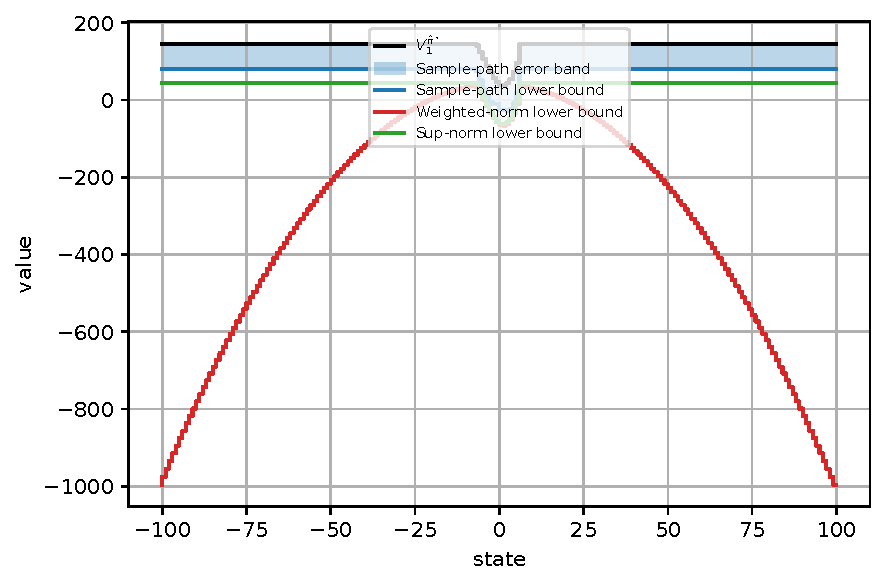
\includegraphics[width=\linewidth]{iot_bounds_zoomed_out.pdf}
    \caption{entire state space}
    \label{fig:iot-out}
  \end{subfigure}
  \hfill
  \begin{subfigure}[b]{0.48\linewidth}
    \centering
    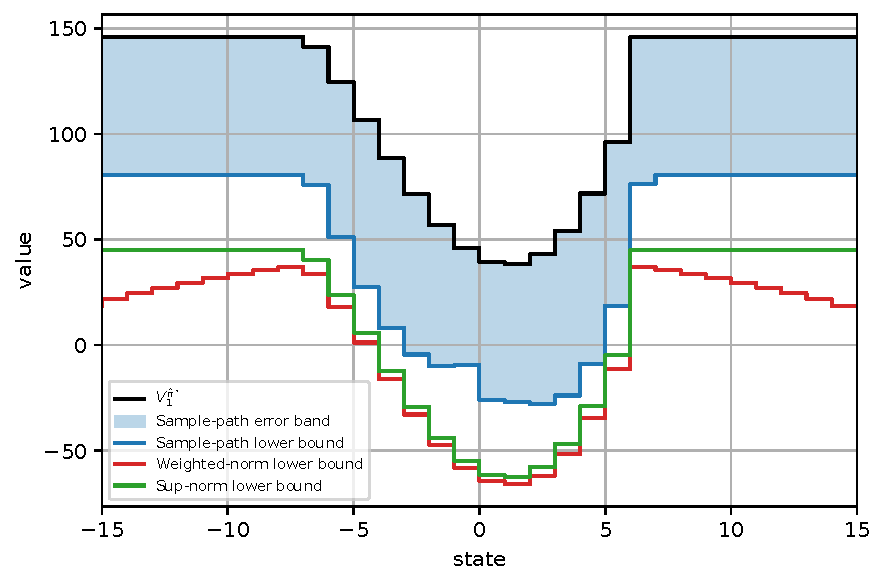
\includegraphics[width=\linewidth]{iot_bounds_zoomed_in.pdf}
    \caption{zoomed in}
    \label{fig:iot-in}
  \end{subfigure}
  \caption{Comparison of lower bounds on $V^\star_1(s)$ for the
    finite-horizon remote transmission-scheduling model.}
  \label{fig:iot-bounds}
\end{figure}

\begin{figure}[t]
  \centering
  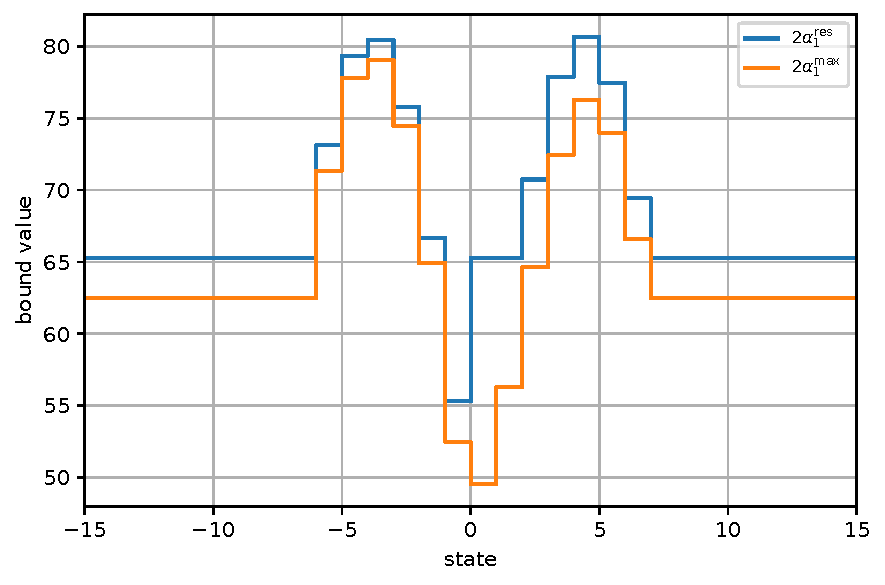
\includegraphics[width=0.6\linewidth]{iot_max_vs_res.pdf}
  \caption{Comparison of $2\alpha^{\max}_1(s)$ and
    $2\alpha^{\mathrm{res}}_1(s)$ in the region
    $s \in \{-15, \dots, 15\}$.}
  \label{fig:iot-max-vs-res}
\end{figure}

\begin{figure}[t]
  \centering
  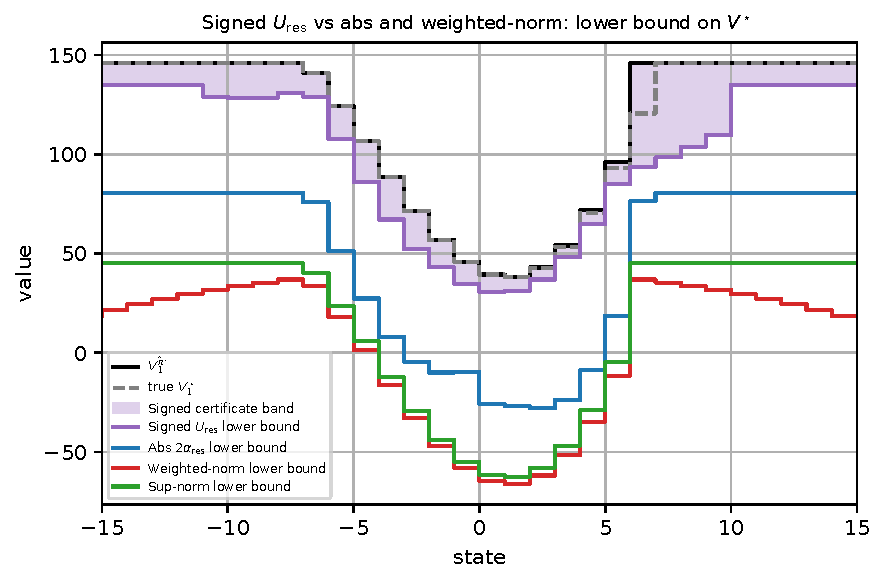
\includegraphics[width=0.6\linewidth]{iot_signed_vs_abs_weighted_zoomed_in.pdf}
  \caption{Signed certificate band
    $[V^{\hat\pi^\star}_1 - U^{\mathrm{res}}_1,\, V^{\hat\pi^\star}_1]$
    versus the absolute-value ($2\alpha^{\mathrm{res}}_1$),
    weighted-norm, and sup-norm lower bounds for the
    transmission-scheduling model, zoomed into the region
    $s \in \{-15, \dots, 15\}$.}
  \label{fig:iot-signed}
\end{figure}

\end{document}
